\chapter{Nuclear physics}
\section{Atomic structure}
\begin{marginfigure}
	\centering
	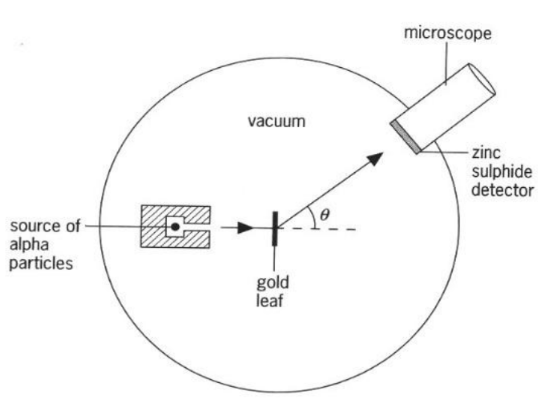
\includegraphics[width=\textwidth]{assets/rutherford-setup.png}
	\caption{Setup of Rutherford scattering}
	\label{fig:rutherford-setup}
\end{marginfigure}
\bf{Why is the vacuum necessary?} \(\alpha\) particles
only travel short distances in air.

Conclusions of Rutherford gold foil experiment:
\begin{marginfigure}
	\centering
	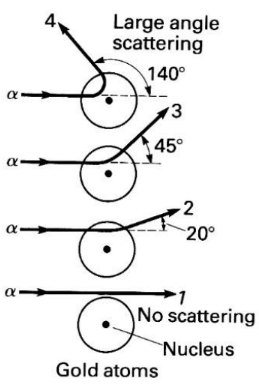
\includegraphics[width=.5\textwidth]{assets/rutherford-scattering.png}
	\caption{Scattering of \(\alpha\) particles}
	\label{fig:rutherford-scattering}
\end{marginfigure}
\begin{itemize}
	\item Large proportion of \(\alpha\) particles are undeflected \(\implies\) most of the atom is empty space
	\item Some \(\alpha\) particles are deflected at small angles \(\implies\) all positive charge and mass is concentrated in a very small volume (the \term{nucleus}!)
	\item Very small proportion of \(\alpha\) particles are deflected at angles more than \qty{90}{\degree} \(\implies\) the nucleus is very small compared to the atom
\end{itemize}

\section{Nuclear reactions}
In nuclear reactions, these must be \it{conserved}:
\begin{itemize}
	\item sum of proton numbers
	\item sum of nucleon numbers
	\item net charge
	\item total momentum\sidenote{for 2 products, momenta are equal in magnitude and opposite in direction!}
	\item total mass--energy
\end{itemize}

Nuclear force is \bf{short-range} and \bf{attractive}, and
falls to 0 at distances greater than \qty{1.5}{\femto\meter}.
\begin{definition}{Binding energy of a nucleus}{binding-energy}
	Energy required to separate the nucleus
	into its consituent free nucleons.
	\\
	{\footnotesize Also equal to energy released when free nucleons are bound together in a nucleus!}
\end{definition}

\begin{definition}{Binding energy per nucleon}{binding-energy-per-nucleon}
	Average energy required to remove a nucleon from the nucleus.
	\\
	{\footnotesize Greater binding energy per nucleon \(\implies\) more stable nucleus!}
\end{definition}

To find \bf{binding energy}, where \(Z\) is the proton number and \(N\) is the neutron number:
\begin{align*}
	\text{binding energy} = E & = \ab(\Delta m)c^2                                \\
	                          & = \ab[\ab(Zm_p + Nm_n) - m_{\text{nucleus}})] c^2
\end{align*}

To find \bf{energy change} of reaction,
\begin{align*}
	\Delta E & = \ab(\sum m_{\text{reactants}} - \sum m_{\text{products}}) c^2        \\
	         & = \sum \text{BE}_{\text{products}} - \sum \text{BE}_{\text{reactants}}
\end{align*}
If the energy change is \it{positive}, energy is released.\sidenote{If no radiation is emitted, released energy is the products' k.e.}
If the energy change is \it{negative}, energy must be supplied (e.g.~through the k.e.~of the reactants) for the reaction to take place.

\section{Radioactivity}
Radioactivity is \bf{spontaneous} and \bf{random}.
\begin{definition}{Spontaneity}{spontaneity}
	Radioactivity is not triggered by external factors/influences;
	rate of decay is unaffected by environmental conditions (e.g.~temperature, pressure).
\end{definition}

\begin{definition}{Randomness}{randomness}
	Impossible to predict which nucleus decays next, or when a particular nucleus will decay.
\end{definition}
Randomness is evidenced by fluctuations in the count rate.

\subsection{Decay types}
A few types of decay in \cref{tab:decay-types}.
\begin{table}[htpb]
	\centering
	\begin{tabular}{r p{0.25\textwidth} p{0.25\textwidth} p{0.25\textwidth}}
		\toprule
		                  & alpha                                                      & beta                                                           & gamma                               \\
		\midrule
		nature of decay   & \(\ce{^4_2He}\) nucleus                                    & \(\ce{^0_{-1}e}\)                                              & photon                              \\
		charge            & \(+2e\)                                                    & \(-e\)                                                         & \(0\)                               \\
		mass              & \qty{4}{\atomicmassunit}                                   & \(m_e\)                                                        & \(0\)                               \\
		penetrating power & easily stopped by paper/skin/a few \unit{\centi\metre} air & stopped by \qty{1}{\metre} air / \qty{3}{\milli\metre} \ce{Al} & several \unit{\centi\metre} \ce{Pb} \\
		\bottomrule
	\end{tabular}
	\caption{Types of decay}
	\label{tab:decay-types}
\end{table}

\begin{itemize}
	\item In \bf{alpha decay}, released energy shows up as the k.e.~of the alpha particle and
	      daughter nucleus. \it{The products have momenta equal in magnitude and opposite in direction.}
	\item In \bf{beta-minus decay}, a neutron in the nucleus transforms into 1 proton and
	      1 electron \ce{^0_{-1}e}; the electron is ejected with some k.e. The remaining k.e.~is
	      present in an \it{antineutrino} \(\bar{\nu}\).
	\item In \bf{beta-plus decay}, a proton in the nucleus transforms into 1 neutron and
	      1 \it{positron} \ce{^0_{+1}e} (charge: \(+e\)). The remaining k.e.~is
	      present in a \it{neutrino} \(\nu\).
\end{itemize}

\section{Measuring decay}
\begin{definition}{Activity}{activity}
	Number of disintegrations per unit time. [\unit{\becquerel} = {\small 1 disintegration \unit{\per\second}}]

	Where \(N \coloneq\) number of radioactive nuclei present,
	\[A = -\odv{N}{t}\]
\end{definition}
Activity cannot be directly measured, so count rate \(C\) is used as a proxy.
\[C \propto A\]
\it{Subtract background count rate} before doing any calculations.

\begin{definition}{Decay constant}{decay-constant}
	The probability per unit time that a nucleus will decay.
	\[R = R_0\exp\ab(-\lambda t)\qquad\text{where}\:R=N, C, A\]
\end{definition}

\begin{definition}{Half-life}{half-life}
	\begin{itemize}
		\item Average time taken for \it{half} the original number of nuclei in a sample to decay \underline{or}
		\item Average time for sample's activity to reduce to \it{half} its original value
	\end{itemize}
	\[t_{\lf{1}{2}} = \f{\ln 2}{\lambda}\]
\end{definition}
